% Usage: knitr slide

\chapter{Hypothesis Testing}\abd{6}
\section{Overview}
Hypothesis testing using traditional frequentist statistical methods
often involves a ``straw man'' hypothesis in an 
attempt to placate reviewers who love $P$-values.  Estimation is more
often appropriate than hypothesis testing.  When hypothesis testing is
really necessary, a choice needs to be made between parametric
(usually Gaussian distribution-based) methods discussed in this
chapter and nonparametric methods to be covered in
Chapter~\ref{chap:nonpar}.  It is not appropriate to use a test of
normality to decide upon a course of action.  Such a strategy would
assume that
\be
\item the test for normality has power near 1.0 for all sample sizes
\item pre-testing for normality does not modify the type I error of
  the testing procedure
\item nonparametric tests are inefficient
\ee
In fact none of these assumptions is true.

We present parametric tests for the following reasons:
\be
\item historical
\item they are very useful for sample size estimation
\item occasionally one has prior information that the raw data, or
  differences from pre to post, actually follow a normal distribution,
  and with large effects one can get quite significant results in very
  small samples with parametric tests
\ee

\section{Hypotheses}
\subsection{Scientific Hypotheses and Questions}
Scientific questions are usually stated with a direction or with
regard to an expected effect, not with respect to a null effect.
Scientific questions often involve estimating a quantify of interest.
Here are some examples:
\bi
\item Does the risk of death increase when serum triglyceride
  increases?
\item Is mechanism $x$ responsible for regulation of physiologic
  parameter $y$?
\item What is the average decrease in blood pressure when the dose of
  a drug goes from 0 to 10mg/day to 20mg/day?
\ei
\subsection{Statistical Hypotheses}
\bi
\item Hypothesis: usually a statement to be judged of the form \\
  ``population value = specified constant''
 \bi
 \item $\mu = 120$mmHg
 \item $\mu_{1} - \mu_{2} = 0$mmHg
 \item Correlation between wealth and religiosity = 0
 \ei
\item Null hypothesis is usually a hypothesis of no effect but can be
 $H_{0}: \mu =$ constant or $H_{0}:$ Probability of heads
 $=\frac{1}{2}$; \\
 $H_{0}$ is often a straw man; something you hope to disprove
\item Alternative hypothesis: $H_1$; e.g.: $H_{1}: \mu \neq 120$mmHg
\item One-sided hypothesis (tested by 1-tailed test): $H_{1}$ is an
  inequality in one direction ($H_{1}: \mu > 120$mmHg)
\item Two-sided hypothesis (2-tailed test, most common type): $H_{1}$
  involves values far from the hypothesized value in either direction
\ei

\section{Branches of Statistics}
\bi
\item Classical (frequentist or sampling statistics)\ros{7.1-7.2}
 \bi
  \item Emphasizes (overemphasizes?) hypothesis testing
 \item Assumes $H_{0}$ is true and tries to amass evidence casting
   doubt on this assumption
 \item Conceives of data as one of many datasets that \emph{might} have
   happened; considers the process by which the sample arose
 \item Inference is based on long-run operating characteristics not
   about direct evidence from the sample at hand
   \bi
   \item false positive probability
   \item probability that varying confidence intervals over replicates
     of the experiment cover the true unknown parameter value a
     certain proportion of the time; no statement about whether the
     current confidence interval covers the true parameter or not
   \ei
 \item See if data are consistent with $H_{0}$
 \item Are data extreme or unlikely if $H_{0}$ is really true?
 \item Proof by contradiction: if assuming $H_{0}$ is true leads to
   results that are ``bizarre'' or unlikely to have been observed,
   casts doubt on premise
 \item Evidence summarized through a single statistic capturing a
   tendency of data, e.g., $\bar{x}$
 \item Look at probability of getting a statistic as or more extreme
   than the calculated one (results as or more impressive than ours)
   if $H_{0}$ is true (the $P$-value)
 \item If the statistic has a low probability of being observed to be
   this extreme we say
   that if $H_{0}$ is true we have acquired data that are very
   improbable, i.e., have witnessed a low probability event
 \item Then evidence mounts against $H_{0}$ and we might reject it
 \item A failure to reject \emph{does not} imply that we have gathered
   evidence in favor of $H_0$ --- many reasons for studies to not
   be impressive, including small sample size ($n$)
 \item Ignores \emph{clinical} significance
 \item Is fraught with how to deal with multiplicity problems
   \bi
   \item No principled recipe for how they should be handled
   \item Arise because
     \bi
     \item type I error is fixed at a number $> 0$
     \item backward time ordering of information
     \ei
   \item Evidence about one question is changed according to whether
     other questions are asked (regardless of their answers)
   \ei
 \ei
\item Classical parametric statistics: assumes the data to arise from
  a certain distribution, often the normal (Gaussian distribution)
\item Nonparametric statistics: does not assume a data distribution;
  generally looks at ranks rather than raw values
\item Bayesian statistics: \ros{7.8}
 \bi
 \item Considers the sample data, not how it arose
 \item Computes the probability that a clinically interesting
   statement is true, e.g. that the new drug lowers population mean
   SBP by at least 5mmHg, given what we observed in the data
 \item More natural and direct approach but requires more work
 \item Because respects forward flow of time/information there is no
   need for nor availability of methods for correcting for
   multiplicity\footnote{Bayesian inference assumes only that the
     prior distribution is ``well calibrated'' in the sense that one
     sticks to the pre-specified prior no matter what information is unveiled.}
 \item Evidence about one question is not tilted by whether other
   questions are asked
 \item Can formally incorporate knowledge from other studies as well
   as skepticism from a tough audience you are trying to convince to
   use a therapy
 \item Starting to catch on (only been available for about 240 years)
   and more software becoming available
 \ei
\item Likelihood inference:
  \bi
  \item Considers the sample data, not how it arose
  \item Akin to Bayesian but without the prior
  \item Interval estimates are based on relative likelihood (from the
    likelihood function) and are called likelihood support intervals
  \item For testing, allows both type I and type II errors
    $\rightarrow 0$ as $n \rightarrow \infty$, whereas with
    frequentist methods the type I error never shrinks as $n
    \rightarrow \infty$
  \item This greatly reduces problems with multiplicities
  \ei
\item Bayesian and likelihood inference use the \emph{likelihood
    principle}; frequentist inference does not 
 \bi
 \item Likelihood principle: All of the evidence in a sample relevant
   to model parameters is in the likelihood function 
 \item If we want to know our current location, frequentist inference
   asks the following: If I am in Nashville, what fraction of routes
   to here involved the southern route I took? 
   There are many paths to get where we are, and frequentists have to
   consider all possible relevant paths.  Bayesian and likelihood
   inference states it differently: Where am I now?  This involves an
   assessment of current evidence about my location.  Asking ``how did
   I get here?'' (i.e., how did the data arise?) involves multiplicity
   issues that answering the simpler question does not. 
\item Consider a sequentially monitored randomized experiment.
  Bayesians and likelihoodists can make infinitely many assessments of
  efficacy with no penalty.  On the other hand, a frequentist must
  think the following way:
  \begin{quote}
    I am at the first interim analysis.  I am going to make later
    assessments of efficacy so I need to discount the current
    assessment and be more conservative or I will spend all my
    $\alpha$ already.\\
    \ldots\\
    I am at the fifth interim analysis.  I made four previous efficacy
    assessments, and even though none of them mattered, I spent
    $\alpha$ so I need to discount the current assessment and be more
    conservative.
 \end{quote}
 \ei
\item We will deal with classical parametric and nonparametric
  statistical tests because of time and because software has evolved further
\ei

\section{Errors in Hypothesis Testing; $P$ Values} \ros{7.2}\katz{7.5.A-7.5.B}
\bi
\item Can attempt to reject a formal hypothesis or just compute
  $P$-value
\item Type I error: rejecting $H_0$ when it is true \\
  $\alpha$ is the probability of making this error (typically set at
  $\alpha=0.05$---for weak reasons)
\item Type II error: failing to reject $H_0$ when it is false \\
  probability of this is $\beta$
\begin{center}
\begin{tabular}{|l||c|c|} \hline
 & \multicolumn{2}{|c|}{True state of $H_0$} \\ \hline 
Decision & $H_0$ true & $H_0$ false \\ \hline \hline
Reject $H_0$ & Type I error ($\alpha$) & Correct \\  \hline
Do Not Reject $H_0$ & Correct & Type II error ($\beta$) \\  \hline
\end{tabular}
\end{center}

\item Power: $1 - \beta$: probability of (correctly) rejecting $H_0$
  when it is false
\ei

Within the frequentist framework of statistics there are two schools.
One, the Neyman-Pearson school, believes that the type I error should
be pre-set at $\alpha$ (say $\alpha=0.05$) so that binary decisions
can be made (reject/fail to reject).  The other school due to Fisher
believes that one should compute $P$-values and quote the result in
the report or publication.  This is the more popular approach, for
good reason.

A $P$-value is something that can be computed without speaking of
errors.  It is the probability of observing a statistic as or more
extreme than the observed one if $H_0$ is true, i.e., if the
population from which the sample was randomly chosen had the
characteristics posited in the null hypothesis.\footnote{Note that
  Rosner's Equation 7.4 in his section 7.3 is highly 
problematic.  Classifications of ``significant'' or ``highly
significant'' are arbitrary, and treating a $P$-value between 0.05 and
0.1 as indicating a ``trend towards significance'' is bogus.  If the
$P$-value is 0.08, for example, the 0.95 confidence interval for the
effect includes a ``trend'' in the opposite (harmful) direction.}

\subsection{Misinterpretation of $P$-values}
$P$-values have come under extreme criticism since 2000, partially
because they are often misinterpreted. Greenland~\etal~\cite{gre16sta}
is the best paper that summarizes the misinterpretations and explains
them.  Some quotes from this paper are below, with their explanations
for the first two.

\begin{quote}
  \begin{enumerate}
  \item \textbf{The $P$ value is the probability that the test
      hypothesis is true; for example, if a test of the null
      hypothesis gave $P$ = 0.01, the null hypothesis has only a 1\%
      chance of being true; if instead it gave $P$ = 0.40, the null
      hypothesis has a 40\% chance of being true.} No! The $P$ value
    assumes the test hypothesis is true---it is not a hypothesis
    probability and may be far from any reasonable probability for the
    test hypothesis. The $P$ value simply indicates the degree to
    which the data conform to the pattern predicted by the test
    hypothesis and all the other assumptions used in the test (the
    underlying statistical model). Thus $P$ = 0.01 would indicate that
    the data are not very close to what the statistical model
    (including the test hypothesis) predicted they should be, while
    $P$ = 0.40 would indicate that the data are much closer to the
    model prediction, allowing for chance variation. 
  \item \textbf{The $P$ value for the null hypothesis is the
      probability that chance alone produced the observed association;
      for example, if the $P$ value for the null hypothesis is 0.08,
      there is an 8\% probability that chance alone produced the
      association.}  No! This is a common variation of the first
    fallacy and it is just as false. To say that chance alone produced
    the observed association is logically equivalent to asserting that
    every assumption used to compute the $P$ value is correct, including
    the null hypothesis. Thus to claim that the null $P$ value is the
    probability that chance alone produced the observed association is
    completely backwards: The $P$ value is a probability computed
    assuming chance was operating alone. The absurdity of the common
    backwards interpretation might be appreciated by pondering how
    the $P$ value, which is a probability deduced from a set of
    assumptions (the statistical model), can possibly refer to the
    probability of those assumptions. Note: One often sees ``alone''
    dropped from this description (becoming ``the $P$ value for the null
    hypothesis is the probability that chance produced the observed
    association''), so that the statement is more ambiguous, but just
    as wrong.
  \item \textbf{A significant test results ($P\leq 0.05$) means that
      the test hypothesis is false or should be rejected.} No!
  \item \textbf{A nonsignificant test results ($P > 0.05$) means that
      the test hypothesis is true or should be accepted.} No!
  \item \textbf{A large $P$ value is evidence in favor of the test
      hypothesis.} No!
  \item \textbf{A null-hypothesis $P$ value greater than 0.05 means
      that no effect was observed, or that absence of an effect was
      shown or demonstrated.} No!
  \item \textbf{Statistical significance indicates a scientifically or
      substantively important relation has been detected.} No!
  \item \textbf{Lack of statistical significance indicates that the
      effect size is small.} No!
  \item \textbf{The $P$ value is the chance of our data occurring if
      the test hypothesis is true; for example, $P$ = 0.05 means that
      the observed association would occur only 5\% of the time under
      the test hypothesis.} No!
  \item \textbf{If you reject the test hypothesis because $P \leq
      0.05$, the change you are in error (the chance your
      ``significant finding'' is a false positive) is 5\%.} No!
  \item \textbf{$P = 0.05$ and $P \leq 0.05$ mean the same thing.} No!
  \item \textbf{$P$ values are properly reported as inequalities (e.g., report ``$P < 0.02$'' when $P = 0.015$ or report $P > 0.05$ when $P = 0.06$ or $P = 0.70$).} No!
  \item \textbf{Statistical significance is a property of the phenomenon being studied, and thus statistical tests detect significance.} No!
  \item \textbf{One should always use two-sided $P$ values.} No!
  \item \textbf{When the same hypothesis is tested in different studies and none or a minority of the tests are statistically significant (all $P > 0.05$), the overall evidence supports the hypothesis.} No!
  \item \textbf{When the same hypothesis is tested in two different populations and the resulting $P$ values are on opposite sides of 0.05, the results are conflicting.} No!
  \item \textbf{When the same hypothesis is tested in two different populations and the same $P$ values are obtained, the results are in agreement.} No!
  \item \textbf{If one observes a small $P$ value, there is a good chance that the next study will produce a $P$ value at least as small for the same hypothesis.} No!
  \item \textbf{The specific 95\% confidence interval presented by a study has a 95\% chance of containing the true effect size.} No!
  \item \textbf{An effect size outside the 95\% confidence interval has been refuted (or excluded) by the data.} No!
  \item \textbf{If two confidence intervals overlap, the difference between the two estimates or studies is not significant.} No!
  \item \textbf{An observed 95\% confidence interval predicts that 95\% of the estimates from future studies will fall inside the observed interval.} No!
  \item \textbf{If one 95\% confidence interval includes the null value and another excludes that value, the interval excluding the null is the more precise one.} No!
  \item \textbf{If you accept the null hypothesis because the null $P$ value exceeds 0.05 and the power of your test is 90\%, the chance you are in error (the chance that your finding is a false negative) is 10\%.} No!
  \item \textbf{If the null $P$ value exceeds 0.05 and the power of this test is 90\% at an alternative, the results support the null over the alternative.} \dots counterexamples are easy to construct \dots
 \end{enumerate}
\end{quote}

\section{One Sample Test for Mean} \ros{7.3-7.4,7.12}
\subsection{Test}
\bi
\item Assuming continuous response from a normal distribution
\item One sample tests for $\mu =$ constant are unusual except when
  data are paired, e.g., each patient has a pre-- and post--treatment
  measurement and we are only interested in the mean of post - pre
  values
\item $t$ tests in general:
\beq
t = \frac{\textrm{estimate - hypothesized value}}{\textrm{standard deviation
  of numerator}}
\eeq
\item The standard deviation of a summary statistic is called its
  \emph{standard error}, which is the $\sqrt{}$ of the variance of the
  statistic 
\item The one-sample $t$ statistic for testing a single population
  mean against a constant $\mu_0$ ($H_{0}$: $\mu = \mu_{0}$; often
  $\mu_{0} = 0$) is 
\beq
t = \frac{\bar{x} - \mu_{0}}{se}
\eeq
where $se = \frac{s}{\sqrt{n}}$, is the standard error of the mean (SEM) and $\bar{x}$ is the sample mean

%because the variance of $\bar{x}$ is the variance of an individual $x$ value divided by the number of values being averaged $\rightarrow \sigma^{2}/n$
% \bi
% \item If you repeated an experiment $M$ times, each time computing
%   $\bar{x}$ from $n$ observations, the $M \bar{x}$s would vary
%   $\frac{1}{n}$th as much as the raw measurements vary between
%   patients
% \ei
\item When your data comes from a normal distribution and $H_{0}$ holds, the
  $t$ ratio follows the $t$ \emph{distribution}
\item With small sample size ($n$), the $t$ ratio is unstable because the sample standard deviation ($s$) is not
  precise enough in estimating the population standard deviation ($\sigma$; we are assuming that $\sigma$
  is unknown)
\item This causes the $t$ distribution to have heavy tails for small
  $n$
\item As $n\uparrow$ the $t$ distribution becomes the normal
  distribution with mean zero and standard deviation one
\item The parameter that defines the particular $t$ distribution to
  use as a function of $n$ is called the \emph{degrees of freedom} or
  d.f.
\item d.f. = $n$ - number of means being estimated
\item For one-sample problem d.f. = $n-1$
\item Symbol for distribution $t_{n-1}$

\begin{Schunk}
\begin{Sinput}
x <- seq(-3, 3, length=200)   # Fig. (*\ref{fig:htest-tpdfs}*)
w <- list(Normal     = list(x=x, y=dnorm(x)),
          't (50 df)'= list(x=x, y=dt(x, 50)),
          't (5 df)' = list(x=x, y=dt(x, 5)),
          't (2 df)' = list(x=x, y=dt(x,2)))
require(Hmisc)
labcurve(w, pl=TRUE, keys='lines', col=c(1,2,4,5), lty=c(2,1,1,1),
         xlab=expression(x), ylab='')
\end{Sinput}
\begin{figure}[htbp]

\centerline{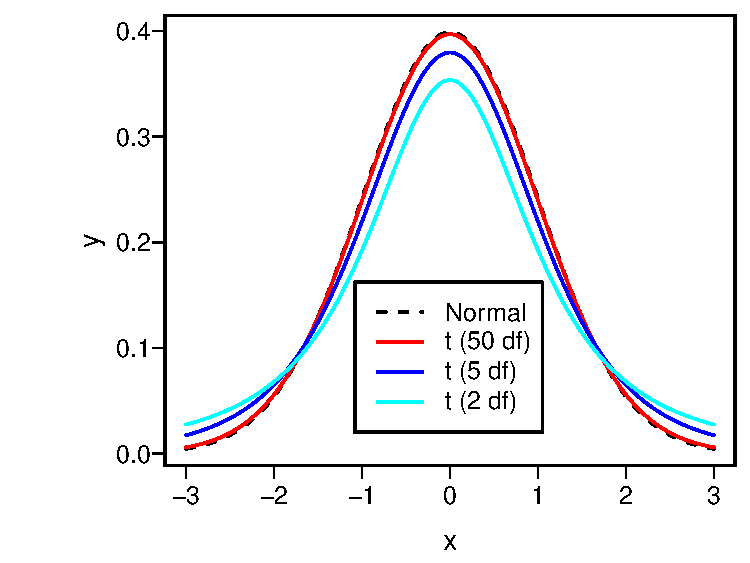
\includegraphics[width=\maxwidth]{htest-tpdfs-1} }

\caption[$t$ distribution for varying d.f.]{Comparison of probability densities for $t_2$, $t_5$, $t_{50}$, and normal distributions}\label{fig:htest-tpdfs}
\end{figure}
\end{Schunk}

\item Two-tailed $P$-value: probability of getting a value from the
  $t_{n-1}$ distribution as big or bigger in absolute value than the
  absolute value of the observed $t$ ratio
\item Computer programs can compute the $P$-value given $t$ and
  $n$.\footnote{\R\ has the function \texttt{pt} for the cumulative
    distribution function for the $t$ distribution, so the 2-tailed
    $P$-value would be obtained using 
    \texttt{2*(1-pt(abs(t),n-1))}.}  See the course web site or go
  to \url{http://surfstat.anu.edu.au/surfstat-home/tables/t.php} for
  an interactive $P$ and critical value calculator for common
  distributions.  But \R\ can compute all probabilities or critical
  values of interest.  See the help files for \co{pt,pnorm,pf,pchisq}.
 \bi
 \item don't say ``$P <$ something'' but instead $P=$ something
 \ei
\item In the old days tables were used to provide \emph{critical
    values} of $t$, i.e., a value $c$ of $t$ such that Prob$[|t| > c]
  = \alpha$ for ``nice'' $\alpha$ such as 0.05, 0.01.
\item Denote the critical value by $t_{n-1;1-\alpha/2}$ for a 2-tailed setup
\item For large $n$ (say $n \geq 500$) and $\alpha=0.05$, this value approximates
  the value from the normal distribution, 1.96
\item Example:  We want to test if the mean tumor volume is 190 mm$^3$ in a population with melanoma, $H_0: \mu = 190$ versus $H_1: \mu \neq 190$.
\beqa
\bar{x}=181.52, s=40, n=100, \mu_{0}=190 \\
t = \frac{181.52 - 190}{40/\sqrt{100}} = -2.12 \\
t_{99,.975}=1.984 \rightarrow \mathrm{reject~at~\alpha=.05} \\
P=0.037
\eeqa
\ei
\begin{Schunk}
\begin{Sinput}
xbar  <- 181.52
s     <- 40
n     <- 100
mu0   <- 190
tstat <- (xbar - mu0) / (s / sqrt(n))
pval  <- 2 * (1 - pt(abs(tstat), n - 1))
c(tstat=tstat, pval=pval)
\end{Sinput}
\begin{Soutput}
      tstat        pval 
-2.12000000  0.03650607 
\end{Soutput}
\end{Schunk}

\subsection{Power and Sample Size} \ros{7.5-7.6}
\bi
\item Power $\uparrow$ when
 \bi
 \item allow larger type I error ($\alpha$; trade-off between type I
   and II errors)
 \item true $\mu$ is far from $\mu_{0}$
 \item $\sigma \downarrow$
 \item $n \uparrow$
 \ei
\item Power for 2-tailed test is a function of $\mu, \mu_{0}$ and
  $\sigma$ only through  $|\mu - \mu_{0}| / \sigma$
\item Sample size to achieve $\alpha=0.05$, power $=0.9$ is approximately
\beq
n = 10.51 \left[\frac{\sigma}{\mu-\mu_{0}}\right]^{2}
\eeq
\item Some power calculators are at \url{statpages.org/#Power}
\item Better: PS program by Dupont and Plummer \url{http://biostat.mc.vanderbilt.edu/PowerSampleSize}

\item Example: The mean forced expiratory volume (FEV) in a population of asthmatics is 2.5 liters per second and the population standard deviation is assumed to be 1.  Determine the number of subjects needed if a new drug is expected to increase FEV to 3.0 liters per second ($\alpha = .05, \beta = 0.1$)
\beqa
\mu=2.5, \mu_0=3, \sigma = 1 \\
n = 10.51 \left[\frac{1}{3-2.5}\right]^{2} = 42.04
\eeqa
  \bi
  \item \textrm{Rounding up, we need 43 subjects to have 0.9 power (42 subjects would have less than 0.9 power)}
  \ei
\ei
\begin{Schunk}
\begin{Sinput}
sigma <- 1
mu    <- 2.5
mu0   <- 3
n     <- 10.51 * (1 / (mu - mu0)) ^ 2
# General formula for approximate power of 1-sample t-test
# Approximate because it uses the normal distribution throughout,
# not the t distribution
alpha <- 0.05
power <- 0.9
delta <- mu - mu0
za    <- qnorm(1 - alpha / 2)
zb    <- qnorm(power)
n     <- ((za + zb) * sigma / delta) ^ 2
c(alpha=alpha, power=power, delta=delta, za=za, zb=zb, n=n)
\end{Sinput}
\begin{Soutput}
    alpha     power     delta        za        zb         n 
 0.050000  0.900000 -0.500000  1.959964  1.281552 42.029692 
\end{Soutput}
\end{Schunk}
A slightly more accurate estimate can be obtained using the $t$
distribution, requiring iterative calculations programmed in \R\
packages such as \co{pwr}.
\begin{Schunk}
\begin{Sinput}
# Make sure pwr package is installed
require(pwr)
\end{Sinput}
\begin{Sinput}
pwr.t.test(d = delta / sigma, power = 0.9, sig.level = 0.05, type='one.sample')
\end{Sinput}
\begin{Soutput}

     One-sample t test power calculation 

              n = 43.99548
              d = 0.5
      sig.level = 0.05
          power = 0.9
    alternative = two.sided
\end{Soutput}
\end{Schunk}

\subsection{Confidence Interval} \ros{R7.7}\altman{28-29}\abd{6.6}
A 2-sided $1-\alpha$ confidence interval for $\mu$ is
\beq
\bar{x} \pm t_{n-1,1-\alpha/2} \times {se}
\eeq
The $t$ constant is the $1-\alpha/2$ level critical value from the
$t$-distribution with $n-1$ degrees of freedom.  For large $n$ it
equals 1.96 when $\alpha=0.05$.

A rough way to interpret this is that we are 0.95 confident that the
unknown $\mu$ lies in the above interval.  The exact way to say it is
that if we were able to repeat the same experiment 1000 times and
compute a fresh confidence interval for $\mu$ from each sample, we
expect 950 of the samples to actually contain $\mu$.  The confidence
level is about the procedure used to derive the interval, not about
any one interval.  Difficulties in
providing exact interpretations of confidence intervals has driven
many people to Bayesian statistics.

The 2-sided $1-\alpha$ CL includes $\mu_{0}$ if and only if a test of $H_{0}:
\mu=\mu_{0}$ is not rejected at the $\alpha$ level in a 2-tailed test.
\bi
\item If a 0.95 CL does not contain zero, we can reject $H_0: \mu = 0$ at the $\alpha = 0.05$ significance level
\ei

$1 - \alpha$ is called the \emph{confidence level} or \emph{confidence
  coefficient}.

\subsection{Sample Size for a Given Precision} \altman{139-148}\abd{14.7}
There are many reasons for preferring to run estimation studies
instead of hypothesis testing studies.  A null hypothesis may be
irrelevant, and when there is adequate precision one can learn from a
study regardless of the magnitude of a $P$-value.  A universal
property of precision estimates is that, all other things being equal,
increasing the sample size by a factor of four improves the precision
by a factor of two.
\bi
\item May want to estimate $\mu$ to within a margin of error of $\pm
  \delta$ with 0.95 confidence\footnote{Adcock~\cite{adc97sam}
    presents both frequentist and Bayesian methods and for precision
    emphasizes solving for $n$ such that the probability of being
    within $\epsilon$ of the true value is controlled, as opposed to
    using confidence interval widths explicitly.}
\item ``0.95 confident'' that a confidence interval includes the true
  value of $\mu$
\item If $\sigma$ were known but we still used the $t$ distribution in
  the formula for the interval, the confidence interval would be
  $\bar{x}\pm \delta$ where
\beq
\delta = \frac{t_{n-1,1-\alpha/2}\sigma}{\sqrt{n}}
\eeq
\item Solving for $n$ we get
\beq
n = \left[\frac{t_{n-1,1-\alpha/2} \sigma}{\delta}\right]^{2}
\eeq
\item If $n$ is large enough and $\alpha=0.05$, required
  $n=3.84[\frac{\sigma}{\delta}]^{2}$
\item Example: if want to be able to nail down $\mu$ to within $\pm
  1$mmHg when the patient to patient standard deviation in blood
  pressure is 10mmHg, $n = 384$
\begin{Schunk}
\begin{Sinput}
sigma <- 10
delta <- 1
3.84 * (sigma / delta) ^ 2
\end{Sinput}
\begin{Soutput}
[1] 384
\end{Soutput}
\end{Schunk}
\item Advantages of planning for precision rather than
  power\footnote{See Borenstein M: \emph{J Clin Epi} 1994;
    47:1277-1285.}
 \bi
 \item do not need to guess the true population value
 \item many studies are powered to detect a miracle and nothing less;
   if a miracle doesn't happen, the study provides \textbf{no} information
 \item planning on the basis of precision will allow the resulting
   study to be interpreted if the $P$-value is 
   large, because the confidence interval will not be so wide as to
   include both clinically significant improvement and clinically
   significant worsening
 \ei
\ei

\section{One Sample Method for a Probability} \ros{7.10}\altman{45-56}\abd{7}
\subsection{Test}
\bi
\item Estimate a population probability $p$ with a sample probability
  $\hat{p}$
\item Approximate 2-sided test of $H_{0}: p=p_{0}$ obtained by
  computing a $z$ statistic
\item A $z$-test is a test assuming that the \emph{test statistic} has
  a normal distribution; it is a $t$-test with infinite ($\infty$) d.f.
\beq
z = \frac{\hat{p} - p_{0}}{\sqrt{p_{0}(1-p_{0})/n}}
\eeq
\item The $z$-test follows the same general form as the $t$-test
\beq
z = \frac{\textrm{estimate - hypothesized value}}{\textrm{standard deviation
  of numerator}}
\eeq
\item Example: $n=10$ tosses of a coin, 8 heads; $H_{0}$: coin is fair
  ($p_{0}=\frac{1}{2}$)
\beq
z = \frac{.8 - .5}{\sqrt{(\frac{1}{2})(\frac{1}{2})/10}} = 1.897
\eeq
\item $P\textrm{-value} = 2 \times$ area under a normal curve to the right of $1.897 =
  2 \times 0.0289 = 0.058$ (this is also the area under the normal
  curve to the right of $1.897$ + the area to the left of $-1.897$)
\begin{Schunk}
\begin{Sinput}
p  <- 0.8
p0 <- 0.5
n  <- 10
z  <- (p - p0) / sqrt(p0 * (1 - p0) / n)
c(z=z, Pvalue=2 * pnorm(-abs(z)))
\end{Sinput}
\begin{Soutput}
         z     Pvalue 
1.89736660 0.05777957 
\end{Soutput}
\end{Schunk}
\item Approximate probability of getting 8 or more or 2 or fewer heads
  if the coin is fair is 0.058
\item Need to use exact methods if $p$ or $n$ is small
\begin{Schunk}
\begin{Sinput}
# Pr(X >= 8) = 1 - Pr(X < 8) = 1 - Pr(X <= 7)
pbinom(2, 10, 0.5) + 1 - pbinom(7, 10, 0.5)
\end{Sinput}
\begin{Soutput}
[1] 0.109375
\end{Soutput}
\begin{Sinput}
# Also compute as the probability of getting 0, 1, 2, 8, 9, 10 heads
sum(dbinom(c(0, 1, 2, 8, 9, 10), 10, 0.5))
\end{Sinput}
\begin{Soutput}
[1] 0.109375
\end{Soutput}
\end{Schunk}
\ei

\subsection{Power and Sample Size}
\bi
\item Power $\uparrow$ as $n \uparrow$, $p$ departs from $p_{0}$, or
  $p_{0}$ departs from $\frac{1}{2}$
\item $n \downarrow$ as required power $\downarrow$ or $p$ departs
  from $p_{0}$
\ei

\subsection{Sample Size for Given Precision}\alabel{sec:htest-p-n}
\bi
\item Approximate 0.95 CL: $\hat{p} \pm 1.96
  \sqrt{\hat{p}(1-\hat{p})/n}$
\item Assuming $p$ is between 0.3 and 0.8, it would not be far off to
  use the worst case standard error $\sqrt{1/(4n)}$ when planning
\item $n$ to achieve a margin of error $\delta$ in estimating $p$: 
\beq
n = \frac{1}{4}\left[\frac{1.96}{\delta}\right]^{2} = \frac{0.96}{\delta^{2}}
\eeq
\item Example: $\delta=.1 \rightarrow n=96$ to achieve a margin of error of
  $\pm 0.1$ with 0.95 confidence
\ei
\begin{Schunk}
\begin{Sinput}
nprec <- function(delta) round(0.25 * (qnorm(0.975) / delta) ^ 2)
nprec(0.1)
\end{Sinput}
\begin{Soutput}
[1] 96
\end{Soutput}
\end{Schunk}

To achive a margin of error of $\pm 0.05$ even in the worst case where
$p=0.5$ one needs $n=384$.

To put this in the context of relative errors, suppose that one wants
to estimate the odds that an event will occur, to within a certain
multiplicative margin of error (MMOE) with 0.95 confidence.  What is
the MMOE as a function of the unknown $p$ when $n=384$?  The standard
error of the log odds is approximately $\sqrt{\frac{1}{n p (1 - p)}}$,
and the half-width of a 0.95 confidence interval for the log odds is
approximately 1.96 times that.  Fix $n=384$ and vary $p$ to get the
MMOE that is associated with the same sample size as a universal
absolute margin of error of 0.05.

\begin{Schunk}
\begin{Sinput}
p <- seq(0.01, 0.99, length=200)
mmoe <- exp(1.96 / sqrt(384 * p * (1 - p)))
plot(p, mmoe, type='l', xlab='Unknown Probability p', ylab='MMOE')
minor.tick()
\end{Sinput}
\begin{figure}[htbp]

\centerline{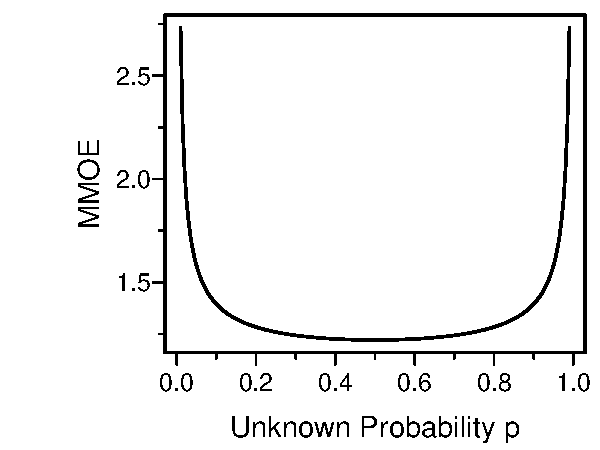
\includegraphics[width=\maxwidth]{htest-moeor-1} }

\caption[Multiplicative margin of error in estimating odds when $n=384$ and the margin of error in estimating the absolute probability is $\leq 0.05$]{Multiplicative margin of error in estimating odds when $n=384$ and the margin of error in estimating the absolute probability is $\leq 0.05$.}\label{fig:htest-moeor}
\end{figure}
\end{Schunk}

\section{Paired Data and One-Sample Tests}  \altman{31-32}\abd{11}
\bi
\item To investigate the relationship between smoking and bone mineral
  density, Rosner presented a paired analysis in which each person had
  a nearly perfect control which was his or her twin
\item Data were normalized by dividing differences by the mean density
  in the twin pair (need to check if this normalization worked)
\item Computed density in heavier smoking twin minus density in
  lighter smoking one
\item Mean difference was $-5\%$ with se=$2.0\%$ on $n=41$
\item The $t$ statistic we've been using works here, once within-pair
  differences are formed
\item $H_{0}:$ mean difference between twins is zero ($\mu_{0} = 0$)
\beqa
t_{40} = \frac{\bar{x} - \mu_{0}}{se} = -2.5 \\
P = 0.0166
\eeqa
\ei
\begin{Schunk}
\begin{Sinput}
xbar  <- -5
se    <- 2
n     <- 41
mu0   <- 0
tstat <- (xbar - mu0) /se
pval  <- 2 * (1 - pt(abs(tstat), n - 1))
c(tstat=tstat, Pvalue=pval)
\end{Sinput}
\begin{Soutput}
      tstat      Pvalue 
-2.50000000  0.01662035 
\end{Soutput}
\end{Schunk}

\section{Two Sample Test for Means} \ros{8}\katz{5.5}\altman{28-35}\abd{12}
\bi
\item Two groups of different patients (unpaired data)
\item Much more common than one-sample tests
\item As before we are dealing for now with parametric tests assuming
  the raw data arise from a normal distribution
\item We assume that the two groups have the same
  spread or variability in the distributions of
  responses\footnote{Rosner covers the unequal variance case very
    well.  As nonparametric tests have advantages for comparing two
    groups and are less sensitive to the equal spread assumption, we
    will not cover the unequal variance case here.}
\ei

\subsection{Test}
\bi
\item Test whether population 1 has the same mean as population 2
\item Example: pop.\ 1=all patients with a certain disease if given
  the new drug, pop.\ 2=standard drug
\item $H_{0}: \mu_{1}=\mu_{2}$ (this can be generalized to test
  $\mu_{1}=\mu_{2}+\delta$, i.e., $\mu_{1}-\mu_{2}=\delta$).  The
  \emph{quantity of interest} or \emph{QOI} is $\mu_{1}-\mu_{2}$
\item 2 samples, of sizes $n_{1}$ and $n_{2}$ from two populations
\item Two-sample (unpaired) $t$-test assuming normality and equal
variances---recall that if we are testing against an $H_0$ of
\textbf{no effect}, the form of the $t$ test is
\beq
t =
\frac{\mathrm{point~estimate~of~QOI}}{\mathrm{se~of~numerator}}
\eeq
\item Point estimate QOI is $\bar{x}_{1} - \bar{x}_{2}$
\item Variance of the sum or difference of two independent means is
  the sum of the variance of the individual means
\item This is $\frac{\sigma^{2}}{n_{1}} + \frac{\sigma^{2}}{n_{2}} =
  \sigma^{2}[\frac{1}{n_{1}} + \frac{1}{n_{2}}]$
\item Need to estimate the single $\sigma^{2}$ from the two samples
\item We use a weighted average of the two sample variances:
\beq
s^{2} = \frac{(n_{1}-1)s^{2}_{1} + (n_{2}-1)s^{2}_{2}}{n_{1}+n_{2}-2}
\eeq
\item True standard error of the difference in sample means: $\sigma
  \sqrt{\frac{1}{n_{1}} + \frac{1}{n_{2}}}$
\item Estimate: $s \sqrt{\frac{1}{n_{1}} + \frac{1}{n_{2}}}$, so
\beq
t = \frac{\bar{x}_{1} - \bar{x}_{2}}{s \sqrt{\frac{1}{n_{1}} + \frac{1}{n_{2}}}}
\eeq
\item d.f.\ is the sum of the individual d.f., $n_{1}+n_{2}-2$, where
  the $-2$ is from our having to estimate the center of two
  distributions
\item If $H_{0}$ is true $t$ has the $t_{n_{1}+n_{2}-2}$ distribution
\item To get a 2-tailed $P$-value we compute the probability that a
  value from such a distribution is farther out in the tails of the
  distribution than the observed $t$ value is (we ignore the sign of
  $t$ for a 2-tailed test)
\item Example: $n_{1}=8, n_{2}=21, s_{1}=15.34, s_{2}=18.23,
  \bar{x}_{1}=132.86, \bar{x}_{2}=127.44$
\beqa
s^{2} &=& \frac{7(15.34)^{2}+20(18.23)^{2}}{7+20} = 307.18 \\
s     &=& \sqrt{307.18} = 17.527 \\
se    &=& 17.527 \sqrt{\frac{1}{8}+\frac{1}{21}} = 7.282 \\
t     &=& \frac{5.42}{7.282} = 0.74
\eeqa
on 27 d.f.
\item $P = 0.463$ (see \R\ code below)
\item Chance of getting a difference in means as larger or larger than
  5.42 if the two populations really have the same means is 0.463
\item $\rightarrow$ little evidence for concluding the population
  means are different
\ei
\begin{Schunk}
\begin{Sinput}
n1    <- 8;         n2 <- 21
xbar1 <- 132.86; xbar2 <- 127.44
s1    <- 15.34;     s2 <- 18.23
s     <- sqrt(((n1 - 1) * s1 ^ 2 + (n2 - 1) * s2 ^ 2) / (n1 + n2 - 2))
se    <- s * sqrt(1 / n1 + 1 / n2)
tstat <- (xbar1 - xbar2) / se
pval  <- 2 * (pt(- abs(tstat), n1 + n2 - 2))
c(s=s, se=se, tstat=tstat, Pvalue=pval)
\end{Sinput}
\begin{Soutput}
         s         se      tstat     Pvalue 
17.5265589  7.2818380  0.7443176  0.4631137 
\end{Soutput}
\end{Schunk}

\subsection{Power and Sample Size}
\bi
\item Power increases when
 \bi
 \item $\Delta = |\mu_{1}-\mu_{2}| \uparrow$
 \item $n_{1} \uparrow$ or $n_{2} \uparrow$
 \item $n_{1}$ and $n_{2}$ are close
 \item $\sigma \downarrow$
 \item $\alpha \uparrow$
 \ei
\item Power depends on $n_{1}, n_{2}, \mu_{1}, \mu_{2}, \sigma$
  approximately through 
\beq
\frac{\Delta}{\sigma \sqrt{\frac{1}{n_{1}}+\frac{1}{n_{2}}}}
\eeq
\item Note that when computing power using a program that asks for
  $\mu_{1}$ and $\mu_{2}$ you can just enter 0 for $\mu_{1}$ and enter
  $\Delta$ for $\mu_{2}$, as only the difference matters
\item Often we estimate $\sigma$ from pilot data, and to be honest we
  should make adjustments for having to estimate $\sigma$ although we
  usually run out of gas at this point
\item Use the \R\ \co{pwr} package, or the power calculator at
  \url{statpages.org/#Power} or PS 
\item Example: \\
 Get a pooled estimate of $\sigma$ using $s$ above (17.52656) \\
% $\sqrt{\frac{15.34^{2}+18.23^{2}}{2}} = 
% 16.847$ when
 Use $\Delta=5, n_{1}=n_{2}=100, \alpha=0.05$
\begin{Schunk}
\begin{Sinput}
delta <- 5
require(pwr)
pwr.t2n.test(n1=100, n2=100, d=delta / s, sig.level = 0.05)
\end{Sinput}
\begin{Soutput}

     t test power calculation 

             n1 = 100
             n2 = 100
              d = 0.2852813
      sig.level = 0.05
          power = 0.5189751
    alternative = two.sided
\end{Soutput}
\end{Schunk}
\item Sample size depends on $k = \frac{n_{2}}{n_{1}}$, $\Delta$, power,
  and $\alpha$
\item Sample size $\downarrow$ when
 \bi
 \item $\Delta \uparrow$
 \item $k \rightarrow 1.0$
 \item $\sigma \downarrow$
 \item $\alpha \uparrow$
 \item required power $\downarrow$
 \ei
\item An approximate formula for required sample sizes to achieve
  power $=0.9$ with $\alpha=0.05$ is
\beqa
n_{1} &=& \frac{10.51 \sigma^{2} (1+\frac{1}{k})}{\Delta^{2}} \\
n_{2} &=& \frac{10.51 \sigma^{2} (1+k)}{\Delta^{2}}
\eeqa
%\item Example using web page: \\
%Does not allow unequal $n_1$ and $n_2$; use power=0.8, $\alpha=0.05,
%\mu_{1}=132.86, \mu_{2}=127.44, \sigma=16.847$
%\item Result is 153 in each group (total=306) vs.\ Rosner's
%  $n_{1}=108, n_{2}=216$, total=324.  The price of having unequal
%  sample sizes was 18 extra patients.
\item Exact calculations assuming normality
\begin{Schunk}
\begin{Sinput}
pwr.t.test(d = delta / s, sig.level = 0.05, power = 0.8)
\end{Sinput}
\begin{Soutput}

     Two-sample t test power calculation 

              n = 193.8463
              d = 0.2852813
      sig.level = 0.05
          power = 0.8
    alternative = two.sided

NOTE: n is number in *each* group
\end{Soutput}
\end{Schunk}
\item If used same total sample size of 388 but did a 2:1
  randomization ratio to get 129 in one group and 259 in the other,
  the power is less
\begin{Schunk}
\begin{Sinput}
pwr.t2n.test(n1 = 129, n2 = 259, d = delta / s, sig.level = 0.05)
\end{Sinput}
\begin{Soutput}

     t test power calculation 

             n1 = 129
             n2 = 259
              d = 0.2852813
      sig.level = 0.05
          power = 0.7519836
    alternative = two.sided
\end{Soutput}
\end{Schunk}
\ei

What is the difference in means that would yield a 2-sided $P$-value
of exactly 0.05 for a two-sample $t$-test with normality and equal
variances when the sample sizes are both equal to $\frac{n}{2}$?  We
solve for $\hat{\Delta} = \bar{x}_{1} - \bar{x}_{2}$ such 
that $t_{n-2,1-\alpha/2} = \frac{\hat{\Delta}}{2s/\sqrt{n}}$, giving
\beq
\hat{\Delta} = \frac{2 \times t_{n-2,1-\alpha/2} \times s}{\sqrt{n}}
\eeq
For total sample sizes of 10, 50, and 100, the ``magic'' values of the
observed difference are the following multiples of the observed
standard deviation $s$:
\begin{Schunk}
\begin{Sinput}
n <- c(10, 50, 100)
tcrit <- qt(0.975, n-2)
2 * tcrit / sqrt(n)
\end{Sinput}
\begin{Soutput}
[1] 1.4584451 0.5686934 0.3968935
\end{Soutput}
\end{Schunk}
Note that these thresholds are independent of the power and the effect
size used in the power calculation.

\subsection{Confidence Interval}  \ros{8.5}\altman{28-35}
\beq
\bar{x}_{1}-\bar{x}_{2} \pm t_{n_{1}+n_{2}-2,1-\alpha/2} \times s \times
\sqrt{\frac{1}{n_{1}} + \frac{1}{n_{2}}}
\eeq
is a $1-\alpha$ CL for $\mu_{1}-\mu_{2}$, where $s$ is the pooled
estimate of $\sigma$, i.e., $s \sqrt{\ldots}$ is the estimate of the
standard error of $\bar{x}_{1}-\bar{x}_{2}$

\subsection{Sample Size for a Given Precision}
To design a study that will nail down the estimate of $\mu_{1}-\mu_{2}$
to within $\pm \delta$ with $1-\alpha$ confidence when $n_{1}=n_{2}=n$, and
when $n$ is large enough so that the critical value
$t_{2n-2,1-\alpha/2}$ may be approximated by the critical value from
the normal distribution, say $z$ ($z=1.96$ when $\alpha=0.05$):
\beq
n = 2\left[\frac{z \sigma}{\delta}\right]^{2}
\eeq
When $\alpha=0.05$, $n = 7.68 [\frac{\sigma}{\delta}]^{2}$

\subsection{Equating Margin of Error to Detectable Difference}
Suppose that a two-arm study is designed to detect a difference $\Delta$ in two
means with power 0.9 at the $\alpha=0.05$ level.  For large enough
sample sizes, the margin of error for estimating the true difference
in means for that study will be $\delta =
\Delta\sqrt{\frac{7.68}{21.02}} = 0.604\Delta$.

\subsection{Checking Assumptions of the $t$-test}
\bi
\item Box plot (one box for each of 2 groups): look for equal spread
  (IQR)
\item Informally compare $s_{1}$ and $s_{2}$\footnote{Rosner 8.6 shows how to
  make formal comparisons, but beware that the variance ratio test
  depends on normality, and it may not have sufficient power to detect
  important differences in variances.}
\item Various plots for assessing normality of data from each
  group\footnote{There are formal tests of normality but in smaller
    samples these may have insufficient power to detect important
    non-normality.}
\ei

\section{The Problem with Hypothesis Tests and $P$-values}
\subsection{Hypothesis Testing}
\bi
\item Existence of ESP is a hypothesis
\item Assessing effects of drugs, procedures, devices involves
  estimation
\item Many studies powered to detect huge effect
\item If effect is not huge, no information from study
\ei

\subsection{$P$-Values} \ros{7.3}\altman{15-24}\abd{6.2}
\bi
\item Only provide evidence against a \emph{null} hypothesis,
  \textbf{never} evidence for something
\item Probability of a statistic as impressive as yours \textbf{\Large
    if} $H_0$ true
\item Not a probability of an effect or difference (same problem with
  sensitivity and specificity)
\item \textbf{No} conclusion possible from large $P$-values
\item Cannot conclude clinical relevance from small $P$
\item Adjustment of $P$-values for multiple tests is controversial and
  there is insufficient consensus on how to choose an adjustment
  method
\ei

\subsection{How Not to Present Results} \abd{6.2}
\bi
\item $P=0.02$ --- let's put this into clinical practice ignoring the
  drug's cost or clinical effectiveness
\item $P=0.4$ --- this drug does not kill people
\item $P=0.2$ but there is a trend in favor of our blockbuster drug
\item The observed difference was 6mmHg and we rejected $H_0$ so the
  true effect is 6mmHg.
\item The proportion of patients having adverse events was 0.01 and
  0.03; the study wasn't powered to detect adverse event differences
  so we present no statistical analysis
\item The reduction in blood pressure was 6mmHg with 0.95 C.L.\ of
  [1mmHg, 11mmHg]; the drug is just as likely to only reduce blood
  pressure by 1mmHg as it is by 6mmHg.
\item The serum pH for the 15 dogs was $7.3 \pm 0.1$ (mean $\pm$ SE)
\ei

\subsection{How to Present Results} \altman{15-24}\abd{6.2}
\bi
\item Estimates should be accompanied by confidence limits
\item Confidence limits can be computed without regard to sample size
  or power
\item A computed value from a sample is only an estimate of the
  population value, whether or not you reject $H_0$
\item Best to think of an estimate from a study as a fuzz, not a point
\item To present variability of subjects, use SD or IQR, \textbf{not}
  SE (SE is the precision of the \emph{mean} of subjects)
\ei

\section{Study Design Considerations}
The major of studies phrased as hypothesis testing experiments are
actually estimation studies, so it is usually preferred to based
sample size justifications on precision (margin of error).  Whether
using effect sizes in power calculations or margins of error in
precision calculations, the quantity of interest should be taken on
the original dependent variable scale or a transformation of it such
as odds or hazard.  

\subsection{Sizing a Pilot Study}
Frequently, pilot studies are used to obtain estimates of variability
that allow the sample sized to be calculated for a full study.  With a
continuous response variable, one can think of the adequacy of the
sample size in terms of the fold change or multiplicative margin of
error (MMOE) in the estimate $s$ of the population standard deviation $\sigma$.

When a sample of size $n$ is
drawn from a normal distribution, a $1 - \alpha$ two-sided confidence confidence
interval for the unknown population variance $\sigma^2$ is
given by
\begin{equation}
  \frac{n-1}{\chi^{2}_{1-\alpha/2,n-1}} s^{2} < \sigma^{2} <
  \frac{n-1}{\chi^{2}_{\alpha/2,n-1}} s^{2},
  \end{equation}
where $s^2$ is the sample variance and $\chi^{2}_{\alpha,n-1}$ is the
$\alpha$ critical value of the $\chi^2$ distribution with $n-1$
degrees of freedom.  The MMOE for estimating $\sigma$ is
\begin{equation}
  \sqrt{\max(\frac{\chi^{2}_{1-\alpha/2,n-1}}{n-1},
  \frac{n-1}{\chi^{2}_{\alpha/2,n-1}})}
\end{equation}
\begin{Schunk}
\begin{Sinput}
n    <- 10:300
low  <- sqrt((n - 1) / qchisq(.975, n - 1))
hi   <- sqrt((n - 1) / qchisq(.025, n - 1))
m    <- pmax(1 / low, hi)
ggplot(data.frame(n, m), aes(x=n, y=m)) + geom_line() +
  ylab('MMOE for s')
nmin <- min(n[m <= 1.2])
\end{Sinput}
\begin{figure}[htbp]

\centerline{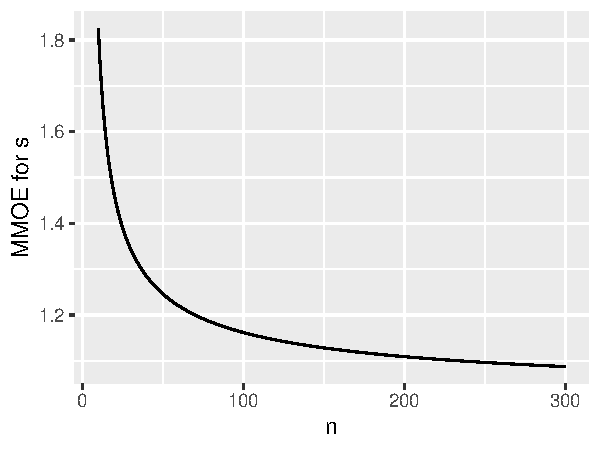
\includegraphics[width=\maxwidth]{htest-smmoe-1} }

\caption[Margin of error in estimating $\sigma$]{Multiplicative margin of error in estimating $\sigma$ as a function of sample size, with 0.95 confidence}\label{fig:htest-smmoe}
\end{figure}
\end{Schunk}
From the above calculations, to achieve a MMOE of no worse than 1.2
with 0.95 confidence when estimating $\sigma$ requires a sample size
of 70 subjects.  A pilot study with $n=20$ will achieve a
MMOE of 1.46 in estimating $\sigma$.

\subsection{Problems with Standardized Effect Sizes}
Many researchers use Cohen's standardized effect sizes in planning a
study. This has the advantage of not requiring pilot data. But such
effect sizes are not biologically meaningful and may hide important
issues~\cite{len01som}. Studies should be designed on the basis
of effects that are relevant to the investigator and human
subjects. If, for example, one plans a study to detect a one standard
deviation (SD) difference in the means and the SD is large, one can
easily miss a biologically important difference that happened to be
much less than one SD in magnitude. Note that the SD is a measure of
how subjects disagree with one another, not a measure of an effect
(e.g., the shift in the mean).  One way to see that standardized
effect sizes are problematic is to note that if one were to make the
measurements more noisy, the SD will increase and the purported
clinically important difference to detect will increase proportionately.

\subsection{Choice of Effect Size}
If a study is designed to detect a certain effect size with a given
power, the effect size should never be the observed effect from
another study, which may be estimated with error and be overly
optimistic. The effect size to use in planning should be the
clinically or biologically relevant effect one would regret
missing.  Usually the only information from prior studies that is
useful in sample size estimation are (in the case of a continuous
response variable with a symmetric distribution) estimates of the
standard deviation or the correlation between two measurements on the
same subject measured at two different times, or (in the case of a
binary or time to event outcome) event probabilities in control
subjects.  An excellent resource by Senn for understanding effect
sizes in power calculations may be found \href{https://errorstatistics.com/2014/03/17/stephen-senn-on-how-to-interpret-discrepancies-against-which-a-test-has-high-power-guest-post/amp}{here}.

\subsection{Multiple Estimands and Hypotheses}
In many experiments there are more than one estimand (what is to be
estimated based on the question of interest) or hypothesis.  Some
frequentist statisticians and biomedical investigators believe that in such
situations the familywise error probability should be
controlled\footnote{As stated elsewhere, multiplicity adjustments are
  a byproduct of faults in frequentist inference and are completely arbitrary.}.
This probability is the probability of rejecting \emph{any} null
hypothesis given that \emph{all} null hypotheses are true.  One may
accomplish this by testing every hypothesis at the $\alpha^{*}$ level,
where the constant $\alpha^{*} < \alpha$ is chosen so that the overall
type one error is $\alpha$, or one may elect to
differentially ``spend $\alpha$'' by, for example, setting $\alpha=0.04$ for a
primary hypothesis and $\alpha=0.01$ for a less important secondary
analysis.  Another alternative is closed testing procedures whereby
later hypotheses can be tested at less stringent $\alpha$ levels as
long as all earlier hypotheses were rejected.  Unfortunately there is
no unique path to deriving multiplicity adjustments, and they have the
odd property of requiring one to be more stringent in assessing
evidence for one hypothesis just because one had other hypotheses.

An alternative, and what we believe to be more reasonable, view is by
Cook and Farewell~\cite{coo96mul} who stated that if a study has more
than one question and each question is to be answered on its own,
there is no need for a multiplicity adjustment.  This is especially
true if a strong priority ordering for hypotheses is stated in
advance.  For example, an investigator may specify three hypotheses about
efficacy of a treatment for the following
endpoints in a cardiovascular trial, sorted from most important to
least important: overall mortality, cardiovascular mortality,
and cardiovascular death or myocardial infarction.  As long as the
researcher always reports all of the results in context, in this
pre-specified order, each $P$-value can stand on its own.

Contrast this with an exploratory study in which the hypothesis is
essentially that there exists an endpoint for which the treatment is
effective.  One should expect to have to employ a conservative
multiplicity adjustment in that situation, e.g., Bonferroni's inequality.

\section{Comprehensive Example: Two sample $t$-test}

\subsection{Study Description}

\bi
\item Compare the effects of two soporific drugs
 \bi
 \item Optical isomers of hyoscyamine hydrobromide
 \ei
\item Parallel-group randomized controlled trial
\item Each subject receives a placebo and then is randomly assigned to receive Drug 1 or Drug 2
\item Dependent variable: Number of hours of increased sleep over
  placebo run-in period.  This should be checked to be a proper change score.

\item Drug 1 given to $n_1$ subjects, Drug 2 given to $n_2$ different subjects
\item Study question: Is Drug 1 or Drug 2 more effective at increasing sleep?
  \bi
  \item $H_0: \mu_1 = \mu_2$
  \item $H_1: \mu_1 \neq \mu_2$
  \ei
\ei

\subsection{Power and Sample Size}

\bi
\item Pilot study or previous published research shows $\sigma = 1.9$ hours
\item Determine the number of subjects needed (in each group) for several value of effect size $\Delta$ ($\Delta = |\mu_1 - \mu_2|$) in order to have 0.9 power with $\alpha = 0.05$
\ei

\begin{table}[!hbp]
 \begin{center}
 \begin{tabular}{lrrrrr} \hline\hline
$\Delta$ &$ 1.0$&$ 1.5$&$ 2.0$&$2.5$ & $3.0$ \\ 
$n$ &$77$&$35$&$20$&$14$&$10$ \\\hline \hline
\end{tabular}
\end{center}

\end{table}

\bi
\item If Drug 1 (or 2) increases sleep by 3.0 hours more than Drug 2 (or 1), by enrolling 10 subjects in each group we will have 0.9 power to detect an association
\ei

\subsection{Collected Data}
\begin{table}[!hbp]
 \begin{center}
 \begin{tabular}{lrr}\hline\hline
Obs. & \multicolumn{1}{c}{Drug 1}&
\multicolumn{1}{c}{Drug 2}
\\ \hline
1 & $ 0.7$&$ 1.9$\\
2 & $-1.6$&$ 0.8$\\
3 & $-0.2$&$ 1.1$\\
4 & $-1.2$&$ 0.1$\\
5 & $-0.1$&$-0.1$\\
6 & $ 3.4$&$ 4.4$\\
7 & $ 3.7$&$ 5.5$\\
8 & $ 0.8$&$ 1.6$\\
9 & $ 0.0$&$ 4.6$\\
10 & $ 2.0$&$ 3.4$\\
& & \\
Mean & $ 0.75$&$ 2.33$\\
SD & $ 1.79$&$ 2.0$\\
\hline
\end{tabular}
\end{center}
\end{table}

\begin{Schunk}
\begin{Sinput}
require(ggplot2)   # Fig (*\ref{fig:htest-sleepa}*)
sleep <- data.frame(drug=c(rep('Drug 1', 10), rep('Drug 2', 10)),
                    extra=c(.7, -1.6, -.2, -1.2, -.1, 3.4, 3.7, .8, 0, 2,
                      1.9, .8, 1.1, .1, -.1, 4.4, 5.5, 1.6, 4.6, 3.4))
ggplot(sleep, aes(x=drug, y=extra, group=drug)) +
  geom_boxplot(col='lightyellow1', alpha=.3, width=.3) + 
  geom_dotplot(binaxis='y', stackdir='center', position='dodge') +
  stat_summary(fun.y=mean, geom="point", col='red', shape=5, size=3) +
  xlab('') + ylab('Extra Hours of Sleep') + coord_flip() 
\end{Sinput}
\begin{figure}[htbp]

\centerline{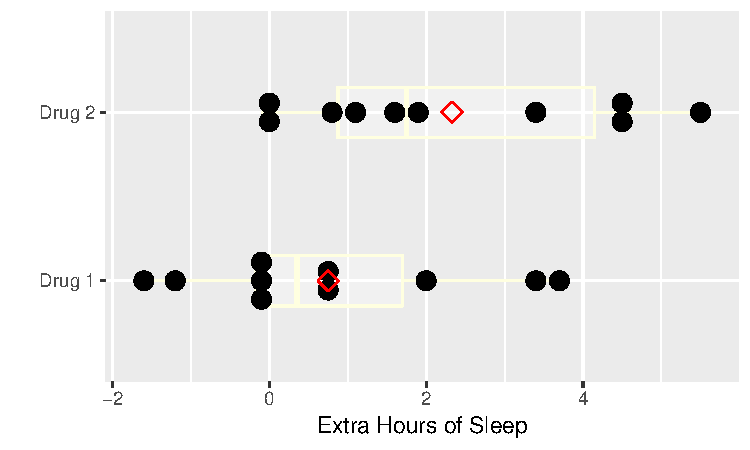
\includegraphics[width=\maxwidth]{htest-sleepa-1} }

\caption[Two-sample parallel group RCT]{Data for two-sample RCT.  Measurements are differences from a control period while subjects were on placebo.  Control period data were not used in the analysis except for normalization.  Diamonds depict means.}\label{fig:htest-sleepa}
\end{figure}
\end{Schunk}

\subsection{Statistical Test}
It is more accepted in practice to now use the form of the $t$-test
that does not assume equal variances in the two independent groups.
The unequal-variance $t$-test is used here.
\begin{Schunk}
\begin{Sinput}
t.test(extra ~ drug, data=sleep)
\end{Sinput}
\begin{Soutput}

	Welch Two Sample t-test

data:  extra by drug
t = -1.8608, df = 17.776, p-value = 0.07939
alternative hypothesis: true difference in means is not equal to 0
95 percent confidence interval:
 -3.3654832  0.2054832
sample estimates:
mean in group Drug 1 mean in group Drug 2 
                0.75                 2.33 
\end{Soutput}
\end{Schunk}
\bi
\item Interpretation
 \bi
 \item Compare Drug 2 to Drug 1.  The output compares 1 to 2
 \item Individuals who take Drug 2 sleep on average 1.58 hours longer (0.95 CI: [-0.21, 3.37]) than individuals who take Drug 1
 \ei
\ei

\clearpage
\section{Comprehensive Example: Paired $t$-test}

\subsection{Study Description}

\bi
\item Compare the effects of two soporific drugs.
\item Crossover study (hopefully with randomized order)
\item Each subject receives placebo run-in, then Drug 1, then Drug 2
\item Investigator did not know about randomized crossover studies
\item Dependent variable: Number of hours of increased sleep when
  compared to a placebo run-in period (raw data not shown)
\item Drug 1 given to $n$ subjects, Drug 2 given to same $n$ subjects
\item Study question: Is Drug 1 or Drug 2 more effective at increasing sleep?
  \bi
  \item $H_0: \mu_d = 0 \hspace{.2cm} \textrm{where} \hspace{.2cm} \mu_d = \mu_1 - \mu_2$
  \item $H_1: \mu_d \neq 0$
  \ei
\ei


\subsection{Power and Sample Size}

\bi
\item Pilot study or previous published research shows the standard deviation of the difference ($\sigma_d$) is $1.2$ hours
\item Determine the number of subjects needed for several value of effect size $\Delta$ ($\Delta = |\mu_1 - \mu_2|$)with 0.9 power, $\alpha = 0.05$
\ei

\begin{table}[!hbp]
 \begin{center}
 \begin{tabular}{lrrrr}\hline\hline
$\Delta$ &$ 0.5$&$ 1$&$1.5$&$2$\\
$n$ &$62$&$16$&$8$&$5$\\
\hline
\end{tabular}
\end{center}
\end{table}

\bi
\item If Drug 1 (or 2) increases sleep by 1.5 hours more than Drug 2 (or 1), by enrolling 8 subjects we will have 0.9 power to detect an association.
\item More powerful than the two sample test (need 10 subjects in each group for $\Delta = 3.0$ hours)
\ei
\subsection{Collected Data}
Here are the data for the 10 subjects.
\begin{table}[!hbp]
 \begin{center}
 \begin{tabular}{lrrr}\hline\hline
Subject & Drug 1 & Drug 2 & {\color{red}Diff (2-1)}
\\ \hline
1 & $ 0.7$&$ 1.9$&$\color{red}1.2$\\
2 &$-1.6$&$ 0.8$&$\color{red}2.4$\\
3 &$-0.2$&$ 1.1$&$\color{red}1.3$\\
4 &$-1.2$&$ 0.1$&$\color{red}1.3$\\
5 &$-0.1$&$-0.1$&$\color{red}0.0$\\
6 &$ 3.4$&$ 4.4$&$\color{red}1.0$\\
7 &$ 3.7$&$ 5.5$&$\color{red}1.8$\\
8 &$ 0.8$&$ 1.6$&$\color{red}0.8$\\
9 &$ 0.0$&$ 4.6$&$\color{red}4.6$\\
10 &$ 2.0$&$ 3.4$&$\color{red}1.4$\\ \\
Mean & $ 0.75$&$ 2.33$&$\color{red}1.58$\\
SD & $ 1.79$&$ 2.0$&$\color{red}1.2$\\
\hline
\end{tabular}\alabel{sleeppaired}
\end{center}
\end{table}
\begin{Schunk}
\begin{Sinput}
drug1 <- c(.7, -1.6, -.2, -1.2, -.1, 3.4, 3.7, .8, 0, 2)
drug2 <- c(1.9, .8, 1.1, .1, -.1, 4.4, 5.5, 1.6, 4.6, 3.4)
d <- data.frame(Drug=c(rep('Drug 1', 10), rep('Drug 2', 10),
                  rep('Difference', 10)),
                extra=c(drug1, drug2, drug2 - drug1))
w <- data.frame(drug1, drug2, diff=drug2 - drug1)

ggplot(d, aes(x=Drug, y=extra)) +   # Fig. (*\ref{fig:htest-tplot}*)
  geom_boxplot(col='lightyellow1', alpha=.3, width=.5) + 
  geom_dotplot(binaxis='y', stackdir='center', position='dodge') +
  stat_summary(fun.y=mean, geom="point", col='red', shape=18, size=5) +
  geom_segment(data=w, aes(x='Drug 1', xend='Drug 2', y=drug1, yend=drug2),
               col=gray(.8)) +
  geom_segment(data=w, aes(x='Drug 1', xend='Difference', y=drug1, yend=drug2 - drug1),
               col=gray(.8)) +
  xlab('') + ylab('Extra Hours of Sleep') + coord_flip() 
\end{Sinput}
\begin{figure}[htbp]

\centerline{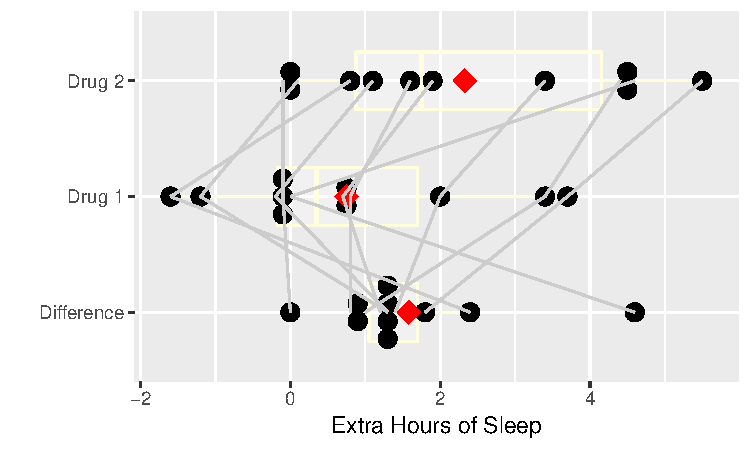
\includegraphics[width=\maxwidth]{htest-tplot-1} }

\caption[Data and box plots for paired data]{Raw data and box plots for paired data and their paired differences, with lines connecting points from the same subject.  Diamonds depict means.}\label{fig:htest-tplot}
\end{figure}
\end{Schunk}

\subsection{Statistical Test}
\begin{Schunk}
\begin{Sinput}
with(d, t.test(drug1, drug2, paired=TRUE))
\end{Sinput}
\begin{Soutput}

	Paired t-test

data:  drug1 and drug2
t = -4.0621, df = 9, p-value = 0.002833
alternative hypothesis: true difference in means is not equal to 0
95 percent confidence interval:
 -2.4598858 -0.7001142
sample estimates:
mean of the differences 
                  -1.58 
\end{Soutput}
\end{Schunk}
\bi
\item Interpretation
 \bi
 \item A person who takes Drug 2 sleeps on average 1.58 hours longer (0.95 CI: [0.70, 2.46]) than a person who takes Drug 1
 \ei
\item Note: Same point estimate (1.58 hours), but more precise estimate (tighter CI) than the 2-sample $t$-test
\ei

\clearpage
\section{Comprehensive Example: Crossover design and analysis}
\bi
 \item In the previous example, it was not clear if the order of placebo, Drug 1, and Drug 2 was the same for every patient
 \item In a cross-over design, each patient receives both drugs
   \bi
     \item Can serve as own control
     \item Order is randomized
   \ei
 \item Carryover effects
   \bi
      \item Def: An effects that carries over from one experimental condition to another
      \item Need a washout period between drugs to remove carryover effects
      \item Time to remove carryover effects should be based on science, not statistics
      \item Statistical tests for carryover effects are often not
        precise enough to make definitive conclusions (see example) 
      \item The test for carryover is correlated with the overall
        test of efficacy
      \item Pre-testing for carryover then deciding whether to only
        use phase 1 data results in a huge inflation of type I error
        in the test for efficacy
   \ei
\ei

\subsection{Study Description}

\bi
\item Compare the effects of two soporific drugs.
\item Each subject either (1) starts with Drug 1 and crosses over to Drug 2 or (2) starts with Drug 2 and crosses over to Drug 1
  \bi
    \item No placebo run-in in this example
    \item Order randomly assigned
    \item Suitable period of time ($\sim 5$ half-lives) between drug
      crossovers to washout effects of previous drug 
  \ei
\item Dependent variable: Number of hours of sleep on each drug
\item Drug 1 given to $n$ subjects, Drug 2 given to same $n$ subjects
\item Study question: Is Drug 1 or Drug 2 more effective at increasing sleep?
  \bi
  \item $H_0: \mu_d = 0 \hspace{.2cm} \textrm{where} \hspace{.2cm} \mu_d = \mu_1 - \mu_2$
  \item $H_1: \mu_d \neq 0$
  \ei
\ei


\subsection{Power and Sample Size}

\bi
\item Pilot study or previous published research shows the standard deviation of the difference ($\sigma_d$) is $1.2$ hours
\item Determine the number of subjects needed for several value of effect size $\Delta$ ($\Delta = |\mu_1 - \mu_2|$)with 0.9 power, $\alpha = 0.05$
\item Assume no carryover effects
\ei

\begin{table}[!hbp]
 \begin{center}
 \begin{tabular}{lrrrr}\hline\hline
$\Delta$ &$ 0.5$&$ 1$&$1.5$&$2$\\
$n$ &$62$&$16$&$8$&$5$\\
\hline
\end{tabular}
\end{center}
\end{table}

\bi
\item If Drug 1 (or 2) increases sleep by 1.5 hours more than Drug 2 (or 1), by enrolling 8 subjects we will have 0.9 power to detect an association.
\item Same power calculation as paired $t$-test
\ei

\subsection{Collected Data}
\begin{table}[!htbp]
 \begin{center}
 \begin{tabular}{lrrr}\hline\hline
Subject & Drug 1 & Drug 2 & {\color{red}Diff (2-1)}
\\ \hline
1  &$8.7$ &$ 9.9$&$\color{red}1.2$\\
2  &$6.4$ &$ 8.8$&$\color{red}2.4$\\
3  &$7.8$ &$ 9.1$&$\color{red}1.3$\\
4  &$6.8$ &$ 8.1$&$\color{red}1.3$\\
5  &$7.9$ &$ 7.9$&$\color{red}0.0$\\
6  &$11.4$&$ 12.4$&$\color{red}1.0$\\
7  &$11.7$&$ 13.5$&$\color{red}1.8$\\
8  &$8.8$ &$ 9.6$&$\color{red}0.8$\\
9  &$8.0$ &$ 12.6$&$\color{red}4.6$\\
10 &$10.0$&$ 11.4$&$\color{red}1.4$\\ \\
Mean&$8.75$&$ 10.33$&$\color{red}1.58$\\
SD  &$1.79$&$ 2.0$  &$\color{red}1.2$\\
\hline
\end{tabular}
\end{center}
\end{table}

\subsection{Statistical Tests}
\begin{Schunk}
\begin{Sinput}
drug1 <- c(87, 64, 78, 68, 79, 114, 117, 88, 80, 100)/10
drug2 <- c(99, 88, 91, 81, 79, 124, 135, 96, 126, 114)/10
t.test(drug1, drug2, paired=TRUE)
\end{Sinput}
\begin{Soutput}

	Paired t-test

data:  drug1 and drug2
t = -4.0621, df = 9, p-value = 0.002833
alternative hypothesis: true difference in means is not equal to 0
95 percent confidence interval:
 -2.4598858 -0.7001142
sample estimates:
mean of the differences 
                  -1.58 
\end{Soutput}
\end{Schunk}
\bi
\item Interpretation
 \bi
 \item A person who takes Drug 2 sleeps on average 1.58 hours longer (0.95 CI: [0.70, 2.50]) than a person who takes Drug 1
 \ei
\ei

\subsection{Carryover Effects}

\bi
   \item Is there any evidence for a carryover effect?
   \item Assume that the first 5 subjects received Drug 1 first and the second 5 subjects received drug 2 first
   \item If we assume there are no carryover effects, then the mean difference in sleep for subjects receiving drug 1 first should be \textit{the same} as the mean difference for subjects receiving drug 2 first
   \item Recall that assessing carryover effect distorts the efficacy
     analysis inference
   \item Null hypothesis is that there are no carryover effects
   \item Can rearrange the difference data to clarify the structure
\ei

\begin{table}[!hbp]
 \begin{center}
 \begin{tabular}{lrr}\hline\hline
Subject & Drug 1 First & Drug 2 First
\\ \hline
1 & $\color{red}1.2$ & \\
2 & $\color{red}2.4$ & \\
3 & $\color{red}1.3$ & \\
4 & $\color{red}1.3$ & \\
5 & $\color{red}0.0$ & \\
6 & & $\color{red}1.0$\\
7 & & $\color{red}1.8$\\
8 & & $\color{red}0.8$\\
9 & & $\color{red}4.6$\\
10 & & $\color{red}1.4$\\ \\
Mean & 1.24 & 1.92 \\
SD & 0.85 & 1.55 \\
\hline
\end{tabular}
\end{center}
\end{table}

For this design we might expect the variance of the differences to be
the same for both orders, so we use the equal-variance $t$-test.
\begin{Schunk}
\begin{Sinput}
# Unpaired t-test
t.test((drug2 - drug1)[1:5], (drug2 - drug1)[6:10], var.equal=TRUE)
\end{Sinput}
\begin{Soutput}

	Two Sample t-test

data:  (drug2 - drug1)[1:5] and (drug2 - drug1)[6:10]
t = -0.86152, df = 8, p-value = 0.414
alternative hypothesis: true difference in means is not equal to 0
95 percent confidence interval:
 -2.500137  1.140137
sample estimates:
mean of x mean of y 
     1.24      1.92 
\end{Soutput}
\end{Schunk}
\bi
\item Interpretation
 \bi
 \item Large $P$-value has no interpretation
 \item With 0.95 confidence, the carryover effect is between [-2.5 and 1.1] hours, which is not scientifically convincing either way
 \item In general, be very cautious when the null hypothesis is something you want to fail to reject in order to validate your analysis method
   \bi
     \item Tests of normality are sometimes used to validate using a parametric over a non-parametric test
     \item There are also statistical tests for equal variance
     \item Both tests promote incorrect interpretation of large
       $P$-value as being evidence supporting the null hypothesis 
   \ei
 \ei
\ei


